\documentclass[tikz,border=3pt]{standalone}
\usepackage{amsmath}
\usetikzlibrary{arrows.meta,shapes.geometric,positioning}

\definecolor{commblue}{RGB}{30,100,225}
\definecolor{senseorange}{RGB}{230,75,35}
\definecolor{controlgray}{RGB}{60,60,60}
\definecolor{apfill}{RGB}{221,230,244}
\definecolor{apedge}{RGB}{31,64,122}
\definecolor{uegreen}{RGB}{25,155,75}

\tikzset{
  control/.style={controlgray,dashed,line width=0.75pt},
  comm/.style={commblue,-{Stealth[length=2.0mm]},line width=0.9pt},
  sense/.style={senseorange,-{Stealth[length=2.0mm]},line width=1.0pt},
  ap/.style={draw=apedge,fill=apfill,rounded corners=1.5pt,line width=0.9pt,
             minimum width=1.12cm,minimum height=0.50cm,font=\sffamily\footnotesize},
  cpu/.style={draw=controlgray,fill=black!4,rounded corners=1.5pt,line width=0.9pt,
              minimum width=2.75cm,minimum height=0.75cm,font=\sffamily\footnotesize,align=center},
  txt/.style={font=\sffamily\footnotesize,align=center},
  note/.style={font=\sffamily\scriptsize,align=center}
}

\begin{document}
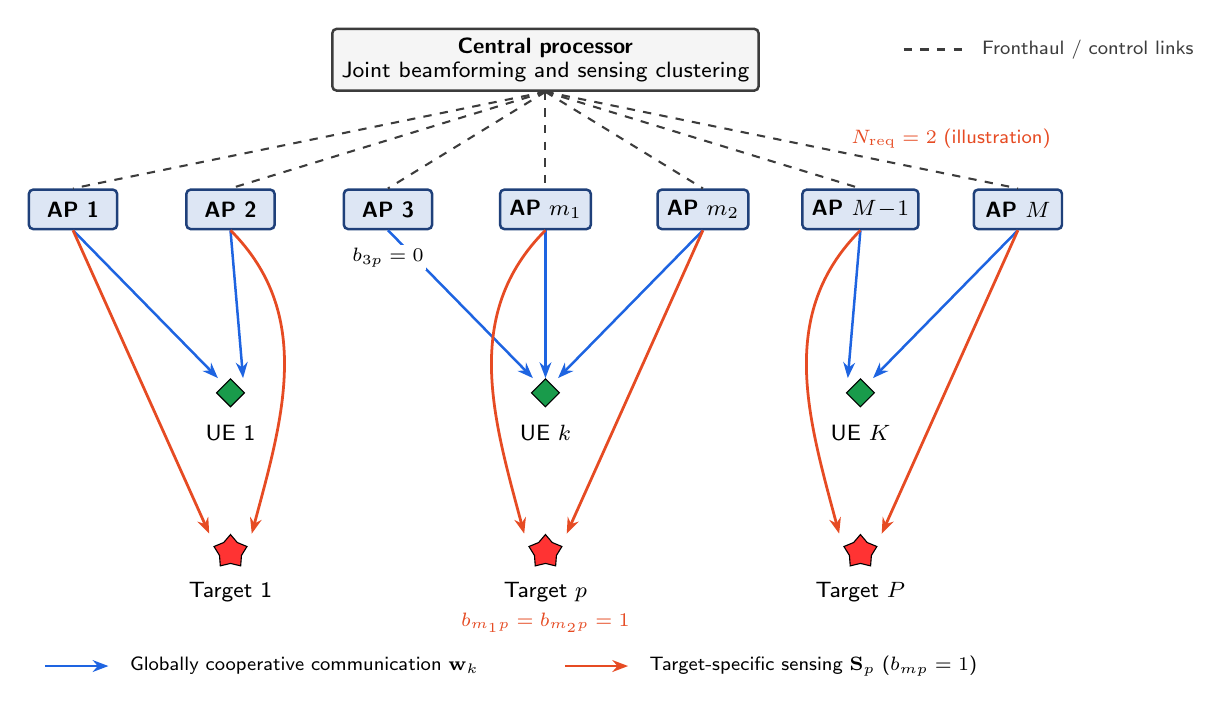
\begin{tikzpicture}[x=1cm,y=1cm]
  % Central coordination and generic AP index set.
  \node[cpu] (cpu) at (0,5.05) {\textbf{Central processor}\\[-1pt]Joint beamforming and sensing clustering};
  \node[ap] (ap1) at (-6.0,3.15) {\textbf{AP 1}};
  \node[ap] (ap2) at (-4.0,3.15) {\textbf{AP 2}};
  \node[ap] (ap3) at (-2.0,3.15) {\textbf{AP 3}};
  \node[ap] (apmone) at (0.0,3.15) {\textbf{AP $m_1$}};
  \node[ap] (apmtwo) at (2.0,3.15) {\textbf{AP $m_2$}};
  \node[ap] (apMmone) at (4.0,3.15) {\textbf{AP $M\! -\! 1$}};
  \node[ap] (apM) at (6.0,3.15) {\textbf{AP $M$}};
  \foreach \a in {ap1,ap2,ap3,apmone,apmtwo,apMmone,apM} {\draw[control] (cpu.south)--(\a.north);}
  \draw[control] (4.55,5.18)--(5.30,5.18);
  \node[note,anchor=west,text=controlgray] at (5.42,5.18) {Fronthaul / control links};

  % Generic user and target index sets.
  \node[diamond,draw=black,fill=uegreen,minimum size=0.36cm,inner sep=0pt] (ue1) at (-4.0,0.82) {};
  \node[diamond,draw=black,fill=uegreen,minimum size=0.36cm,inner sep=0pt] (uek) at (0.0,0.82) {};
  \node[diamond,draw=black,fill=uegreen,minimum size=0.36cm,inner sep=0pt] (ueK) at (4.0,0.82) {};
  \node[txt,below=3pt] at (ue1.south) {UE 1};
  \node[txt,below=3pt] at (uek.south) {UE $k$};
  \node[txt,below=3pt] at (ueK.south) {UE $K$};
  \node[star,star points=5,draw=black,fill=red!80,minimum size=0.44cm,inner sep=0pt] (t1) at (-4.0,-1.20) {};
  \node[star,star points=5,draw=black,fill=red!80,minimum size=0.44cm,inner sep=0pt] (tp) at (0.0,-1.20) {};
  \node[star,star points=5,draw=black,fill=red!80,minimum size=0.44cm,inner sep=0pt] (tP) at (4.0,-1.20) {};
  \node[txt,below=3pt] at (t1.south) {Target 1};
  \node[txt,below=3pt] at (tp.south) {Target $p$};
  \node[txt,below=3pt] at (tP.south) {Target $P$};

  % Representative AP-to-UE communication beams; no b_mp gating.
  \draw[comm] (ap1.south)--([xshift=-1.6mm]ue1.north);
  \draw[comm] (ap2.south)--([xshift=1.6mm]ue1.north);
  \draw[comm] (ap3.south)--([xshift=-1.6mm]uek.north);
  \draw[comm] (apmone.south)--(uek.north);
  \draw[comm] (apmtwo.south)--([xshift=1.6mm]uek.north);
  \draw[comm] (apMmone.south)--([xshift=-1.6mm]ueK.north);
  \draw[comm] (apM.south)--([xshift=1.6mm]ueK.north);
  \node[note,fill=white,inner sep=1pt] at (-2.0,2.54) {$b_{3p}=0$};

  % A consistent N_req=2 sensing example. Every orange curve starts at one AP
  % and ends at one target, and is routed around the UE icons.
  \draw[sense] (ap1.south)--([xshift=-2.7mm]t1.north);
  \draw[sense] (ap2.south) to[out=-45,in=75] ([xshift=2.7mm]t1.north);
  \draw[sense] (apmone.south) to[out=-135,in=105] ([xshift=-2.7mm]tp.north);
  \draw[sense] (apmtwo.south)--([xshift=2.7mm]tp.north);
  \draw[sense] (apMmone.south) to[out=-135,in=105] ([xshift=-2.7mm]tP.north);
  \draw[sense] (apM.south)--([xshift=2.7mm]tP.north);
  \node[note,text=senseorange] at (5.15,4.05) {$N_{\mathrm{req}}=2$ (illustration)};
  \node[note,text=senseorange,fill=white,inner sep=1pt] at (0,-2.10)
      {$b_{m_1p}=b_{m_2p}=1$};

  % Compact legend.
  \draw[comm] (-6.35,-2.65)--(-5.55,-2.65);
  \node[note,anchor=west] at (-5.40,-2.65) {Globally cooperative communication $\mathbf{w}_k$};
  \draw[sense] (0.25,-2.65)--(1.05,-2.65);
  \node[note,anchor=west] at (1.20,-2.65) {Target-specific sensing $\mathbf{S}_p$ ($b_{mp}=1$)};
\end{tikzpicture}
\end{document}
